\chapter{Classification} \label{chap:chap-3}


% add citation for the chapter if it is a reprint


% remove the following and add your chapter text
\section{Introduction}
Classifying the experiments based on the metals and ligands used is explored to further demonstrate the feasibility of using this encoding technique for various machine learning tasks. An important insight to consider is the similarity between voltammetry data and images. After all, each point has a potential and current value, which is similar to an image's RGB values. The main difference is that an image is 2-dimensional while voltammetry data is 1-dimensional. Many previous works have used convolutional neural networks for classification tasks \cite{SHARMA2018377}. Using this as inspiration, the proposed model architecture for voltammetry data classification uses 1-dimensional convolutional layers.  
It is important to note that the dataset used only contains 800 CV datapoints and 200 DPV datapoints for a total of 1000. For training, the dataset was split with 80\% for training, 10\% for validation, and 10\% for testing. 
\section{Variational Autoencoders}
Since one of the large challenges faced is the dataset size, one method to address this is to create synthetic data. 
A variational autoencoder (VAE) is similar to an autoencoder neural network architecture with the main difference being that VAEs connects the encoder to its decoder through a probabilistic latent space that corresponds to the parameters of a variational distribution \cite{PinheiroCinelli2021}. The encoder maps each point from the dataset into a distribution within the latent space rather than a single point in that space. The distribution is typically Gaussian with a mean and a variance. Once the VAE is trained, different points can be sampled from the learned latent space distribution. These samples represent different configurations of the input data in the latent space. The sampled points from the latent space are then fed into the decoder network, which generates reconstructions of the input data corresponding to those points. By sampling multiple points from the latent space and decoding them, a diverse set of synthetic data samples that resemble the original data distribution is generated. The variability in the latent space allows for the generation of novel and diverse data samples that capture the underlying characteristics of the training data.
\section{Conditional Variational Autoencoders}
While traditional VAEs learn a latent space for the dataset, conditional variational autoencoders (CVAEs) expand this concept by introducing conditional dependencies between the input data and the latent variables. In the context of generating synthetic data, CVAEs offer a more controlled approach by allowing the generation process to be conditioned on additional information, such as class labels or other attributes associated with the data.
By conditioning the generation process on known attributes or labels, CVAEs can generate synthetic data samples that not only capture the underlying data distribution but also adhere to specific conditions or constraints defined by the conditioning variables. This enables targeted generation of synthetic data for different classes or categories, even in the absence of labeled data. In this case, the metal and ligand are encoded using one-hot encoding and passed to the decoder to generate data belonging to the same class. 
\section{Classifier Model Architecture}
The model consists of several convolutional layers followed by max-poolling layers to encode the data and reduce dimensions. All layers except for the output layer use the ReLU activation function. The output layer is a dense layer with 10 units and softmax activation function. The Adam optimizer and categorical cross-entropy loss are used to train the model. Additionally, the model uses L2 regularization and early stopping to prevent overfitting and ensure smooth convergence. The Glorot uniform initializer is used for weight initialization to facilitate better gradient flow and prevent exploding gradients. 
\begin{figure}[!h]
  \centering
    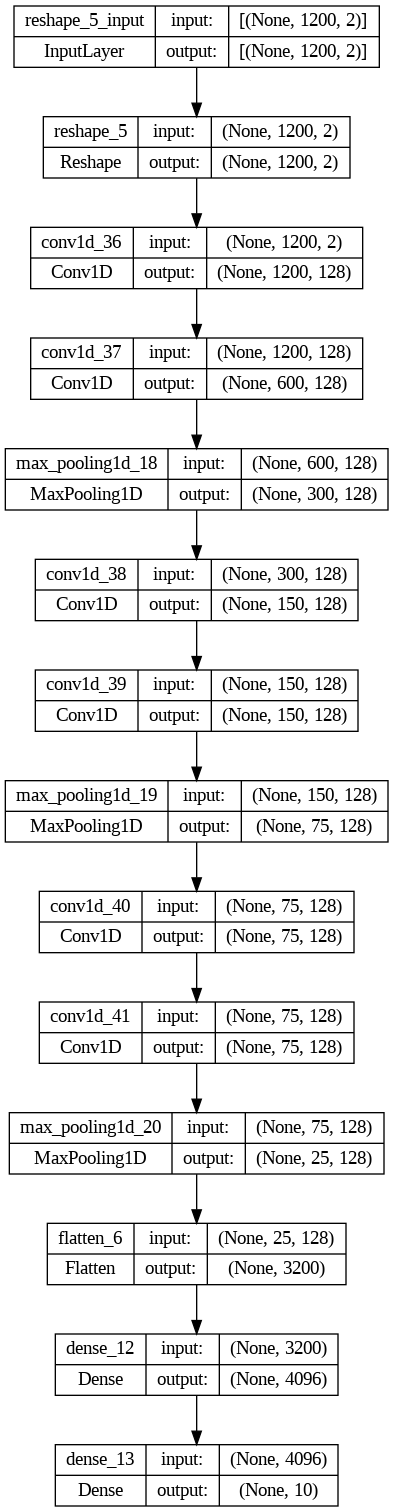
\includegraphics[width=0.25\textwidth]{figures/model_architecture.png}
    \caption{Classification Model Architecture}
    \label{model_arch}
\end{figure}
\section{Results and Discussion}
\begin{table}[!h]
\begin{center}
\begin{tabular}{c|c}
Model & Accuracy (\%) \\
\hline
CV Ligands & 75.13\% \\
CV Metals & 79.24\% \\
DPV Ligands & 30.00\% \\
DPV Metals & 15.87\%
\end{tabular}
\caption{Classification Results}
\end{center}
\end{table}
The accuracy of the classifiers were much better for the CV data compared to the DPV data. This difference can likely be attributed to the size of the datasets. 
\begin{table}[!h]
\begin{center}
\begin{tabular}{c|c}
Model & Accuracy (\%) \\
\hline
CV Ligands & 77.86\% \\
CV Metals & 85.00\% \\
DPV Ligands & 29.34\% \\
DPV Metals & 13.85\%
\end{tabular}
\caption{Classification Accuracy with Synthetic Data}
\end{center}
\end{table}
Similarly after incorporating synthetic data generated with the CVAE into the training process, there was an significant improvement in accuracy for classifying CV data. However, the DPV classifiers actually saw a decrease in performance. Again, this is likely due to the size of the dataset. In utilizing Variational Autoencoders (VAEs) to generate synthetic data, several key considerations impact classifier performance, especially when dealing with small datasets. Firstly, the quality and diversity of the original data influence the effectiveness of the synthetic data produced by VAEs. With limited variation or complexity in a small dataset, the VAE might struggle to capture the true underlying data distribution accurately, potentially resulting in synthetic data that fails to fully represent the characteristics of the real data. This mismatch can detrimentally affect classifier performance. Additionally, the risk of overfitting is heightened in small datasets, where the classifier may excessively specialize on training data patterns that do not generalize well. Introducing synthetic data from a VAE can compound this issue if the VAE itself overfits to the small dataset, producing synthetic data overly similar to the training data, which provides minimal additional information for the classifier and can lead to decreased performance on unseen data. VAEs implicitly learn the probability distribution of the input data. However, if the distribution of the real data is significantly different from the distribution learned by the VAE due to the small dataset size, the synthetic data generated by the VAE may not accurately represent the true data distribution. This distribution mismatch can confuse the classifier, as it may encounter data points in the synthetic dataset that deviate from the real data distribution, leading to suboptimal performance.
\begin{table}[!h]
\begin{center}
\begin{tabular}{c|c|c|c|c}
 & Precision & Recall & F1-Score & Support\\
\hline
Metal 1 & 0.88 & 0.88 & 0.88 & 8\\
Metal 2 & 0.80 & 1.00 & 0.89 & 8\\
Metal 3 & 1.00 & 1.00 & 1.00 & 4\\
Metal 4 & 1.00 & 0.83 & 0.91 & 12\\
Metal 5 & 1.00 & 0.71 & 0.83 & 7\\
Metal 6 & 0.88 & 0.78 & 0.82 & 9\\
Metal 7 & 0.82 & 0.90 & 0.86 & 10\\
Metal 8 & 0.50 & 0.40 & 0.44 & 5\\
Metal 9 & 0.78 & 1.00 & 0.88 & 7\\
Metal 10 & 0.82 & 0.90 & 0.86 & 10\\
\hline
Accuracy & & & 0.85 & 80\\
Macro Avg & 0.85 & 0.84 & 0.84 & 80\\
Weighted Avg & 0.86 & 0.85 & 0.85 & 80
\end{tabular}
\caption{CV Metals Classification Report}
\label{cv_metal_report}
\end{center}
\end{table}
Table \ref{cv_metal_report} provides insights into the precision, recall, and F1-score of each metal type classification, along with the number of instances (support) for each metal type. Precision indicates the proportion of true positive predictions among all positive predictions, while recall measures the proportion of true positives that were correctly identified. F1-score, the harmonic mean of precision and recall, provides a balanced measure between the two.
Overall, the classifier model achieved an accuracy of 85\%, indicating its effectiveness in classifying different metal types. However, it is important to note variations in performance across metal types. For instance, Metal 3 achieved perfect precision, recall, and F1-score, suggesting the model's excellent ability to classify this particular metal type accurately. On the other hand, Metal 8 exhibited lower precision and recall scores, indicating potential challenges in accurately distinguishing this metal type from others.
In terms of macro-average and weighted-average metrics, both hover around 0.85, indicating a reasonably balanced performance across all metal types. These metrics consider the average performance across all classes, with macro-average treating all classes equally, while weighted-average considers the contribution of each class based on its support.
\begin{table}[!h]
\begin{center}
\begin{tabular}{c|c|c|c|c}
 & Precision & Recall & F1-Score & Support\\
\hline
Ligand 1 & 0.88 & 0.78 & 0.82 & 9\\
Ligand 2 & 0.88 & 0.88 & 0.88 & 8\\
Ligand 3 & 0.75 & 0.86 & 0.80 & 7\\
Ligand 4 & 0.45 & 0.71 & 0.56 & 7\\
Ligand 5 & 0.78 & 0.70 & 0.74 & 10\\
Ligand 6 & 1.00 & 0.86 & 0.92 & 7\\
Ligand 7 & 0.71 & 0.50 & 0.59 & 10\\
Ligand 8 & 0.67 & 0.89 & 0.76 & 9\\
Ligand 9 & 1.00 & 0.67 & 0.80 & 3\\
Ligand 10 & 1.00 & 0.90 & 0.95 & 10\\
\hline
Accuracy & & & 0.78 & 80\\
MacroAvg & 0.81 & 0.77 & 0.78 & 80\\
WeightedAvg & 0.80 & 0.78 & 0.78 & 80
\end{tabular}
\caption{CV Ligands Classification Report}
\label{cv_metal_report}
\end{center}
\end{table}
Table \ref{cv_metal_report} shows the classification report for classifying ligands. The classifier achieved an accuracy of 78\% overall, indicating its capability to classify different metal types to some extent. However, upon closer examination, there are notable variations in performance across metal types. For instance, Metal 6 demonstrates excellent precision, recall, and F1-score, suggesting the model's proficiency in accurately classifying this metal type. Conversely, Metal 4 exhibits lower precision, recall, and F1-score, indicating challenges in effectively distinguishing this metal type from others.
\begin{figure}[h!]
  \centering
    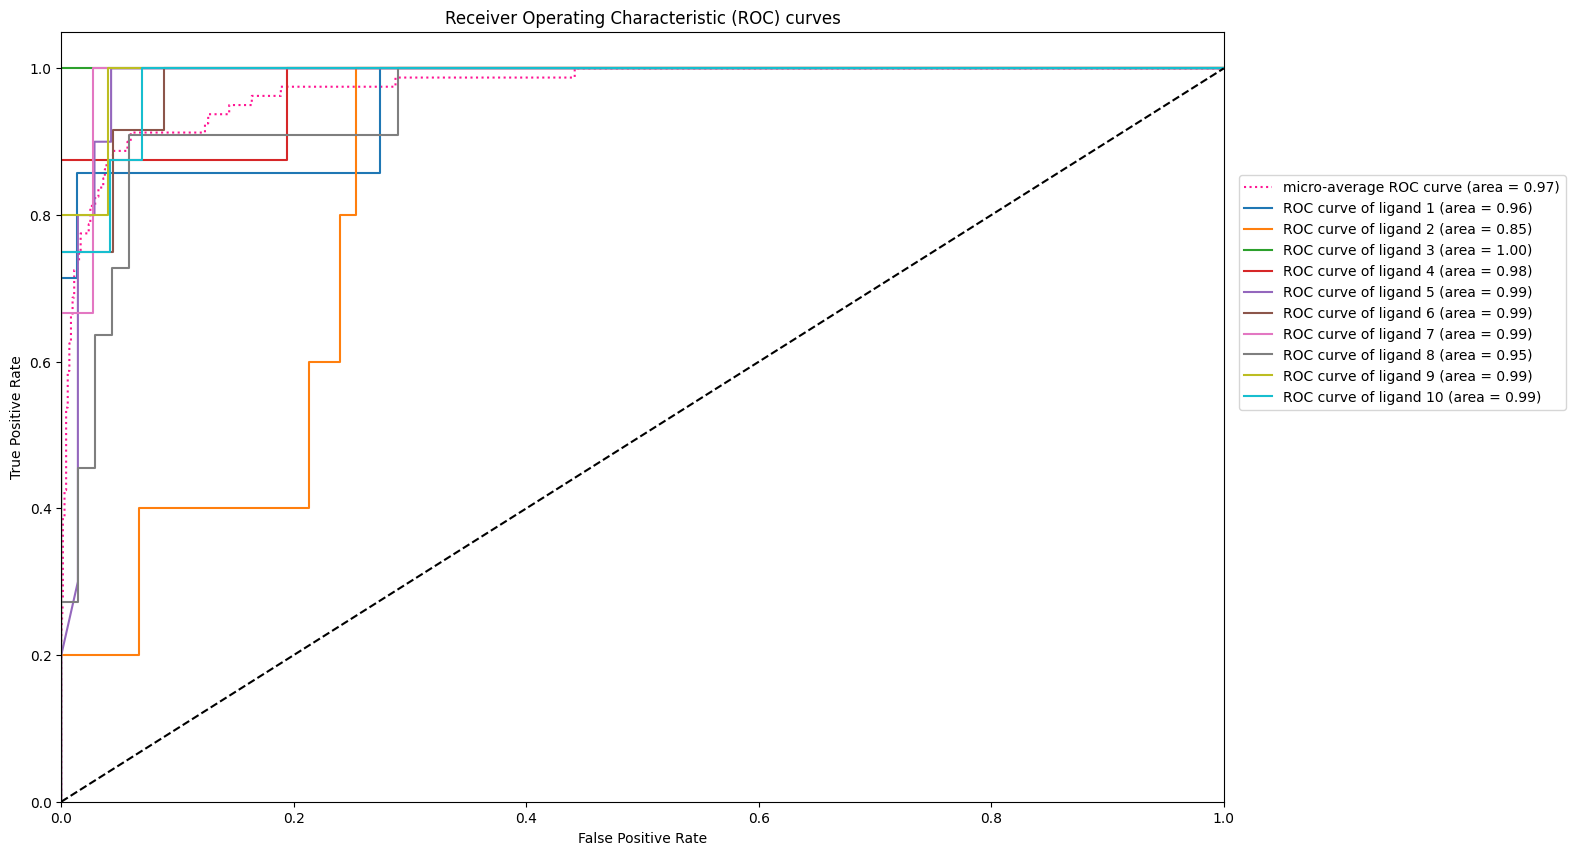
\includegraphics[width=1.0\textwidth]{figures/ligand_roc.png}
    \caption{CV Ligand ROC Curves}
    \label{ligand_roc}
\end{figure}
\begin{figure}[h!]
  \centering
    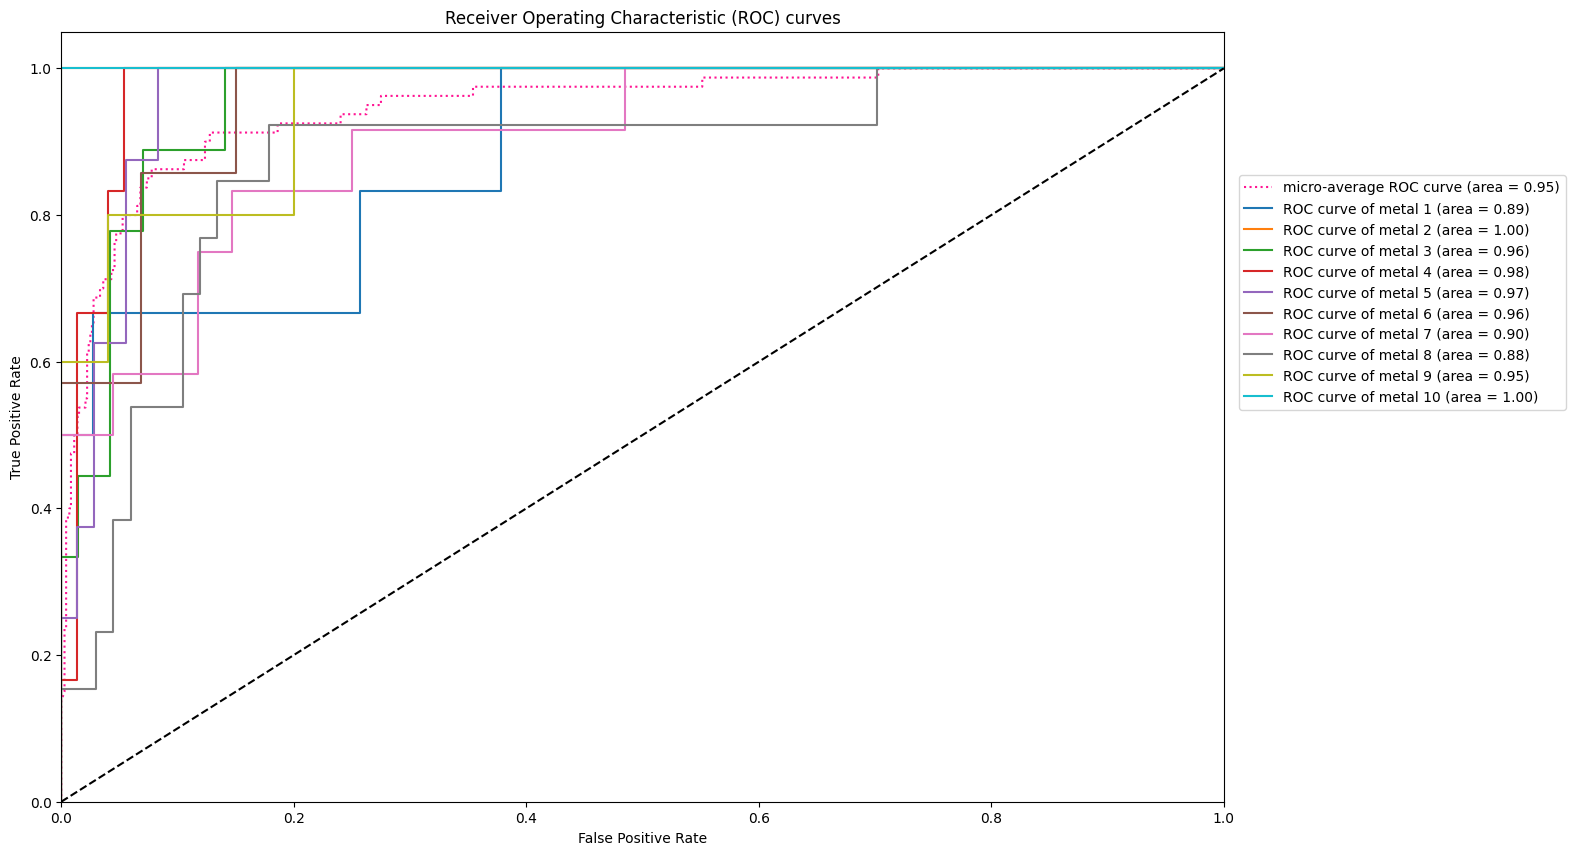
\includegraphics[width=1.0\textwidth]{figures/metal_roc.png}
    \caption{CV Metal ROC Curves}
    \label{metal_roc}
\end{figure}
The area under receiving operating characteristic (ROC) curve shows good results for both metals and ligands. The area under the ROC curve (AUC) calculation summarized the ROC curve analysis into a scalar value, which ranges between 0 and 1. The closer the AUC score to value 1, the better the application’s overall performance.
\begin{figure}[h!]
  \centering
    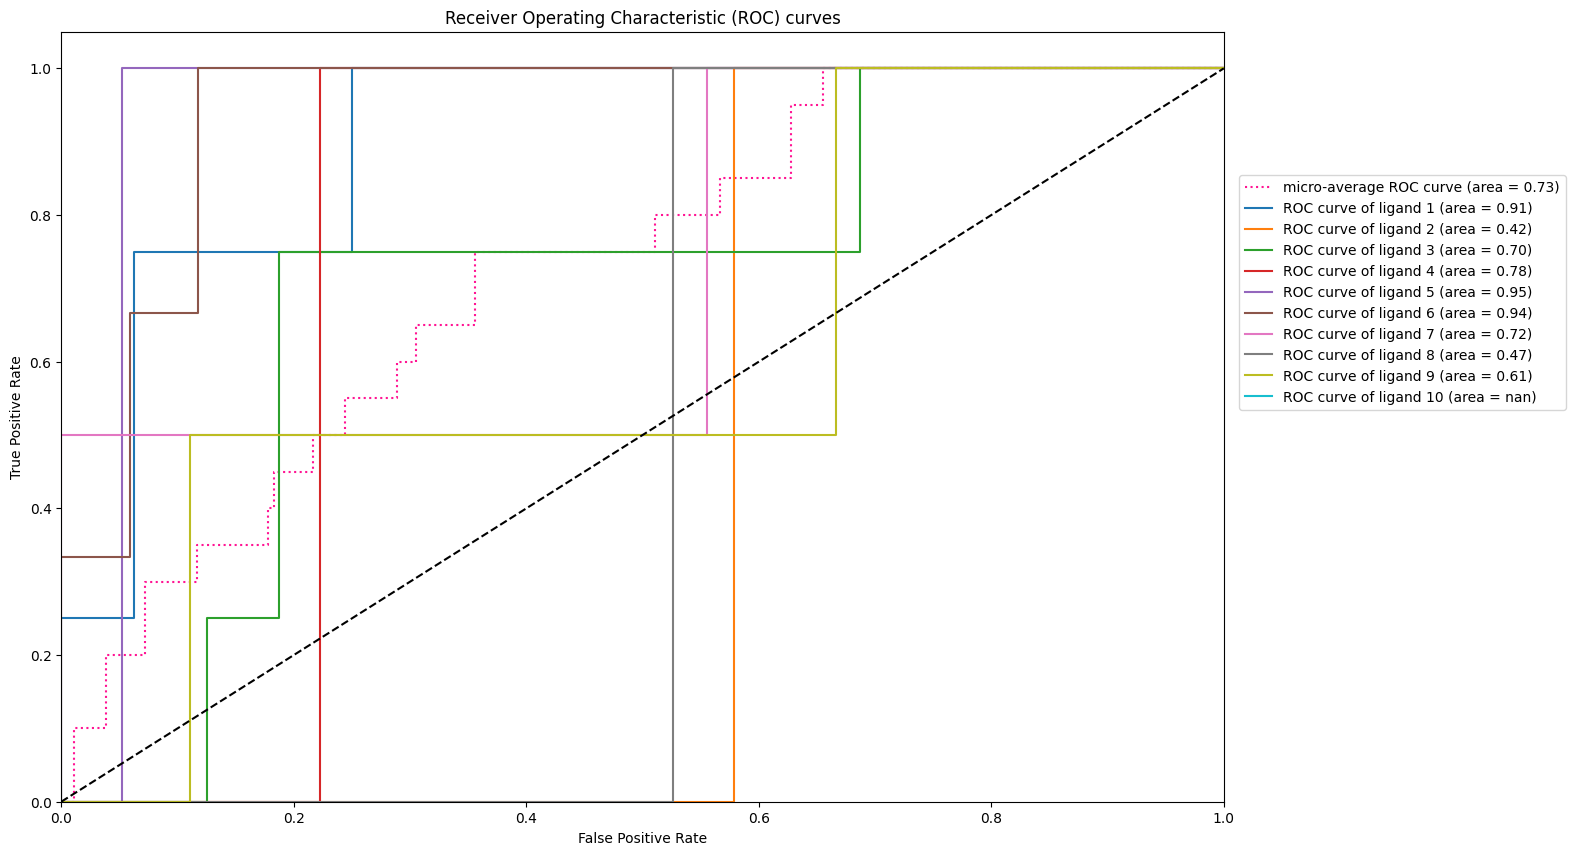
\includegraphics[width=1.0\textwidth]{figures/dpv_ligand_roc.png}
    \caption{DPV Ligand ROC Curves}
    \label{dpv_ligand_roc}
\end{figure}
\begin{figure}[h!]
  \centering
    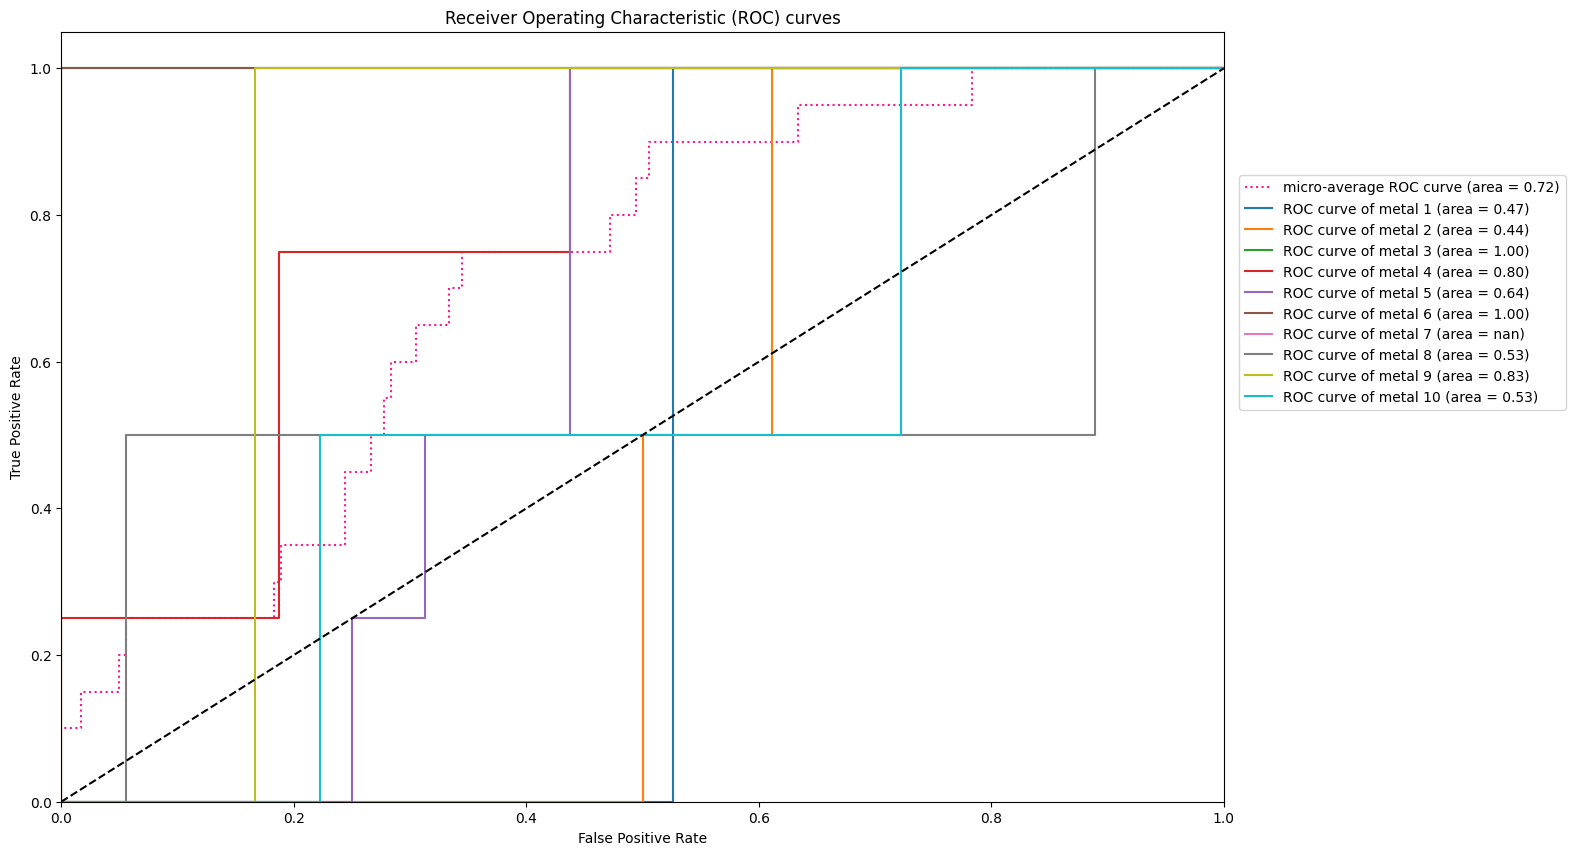
\includegraphics[width=1.0\textwidth]{figures/dpv_metal_roc.png}
    \caption{DPV Metal ROC Curves}
    \label{dpv_metal_roc}
\end{figure}
In Figure \ref{dpv_ligand_roc} and Figure \ref{dpv_metal_roc}, the ROC curves show that the classifier outperform a random classifier by having a AUC value above 0.5. 
\begin{figure}[h!]
  \centering
    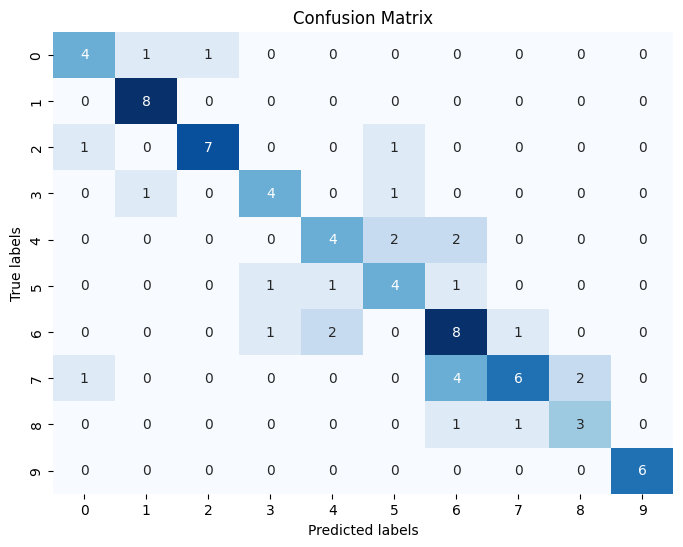
\includegraphics[width=1.0\textwidth]{figures/cv_ligand_matrix.png}
    \caption{CV Ligand Confusion Matrix}
    \label{cv_ligand_matrix}
\end{figure}
From the confusion matrix for ligands \ref{cv_ligand_matrix}, metal 7 was difficult to recognize and was often misclassified as metal 6. 
\begin{figure}[h!]
  \centering
    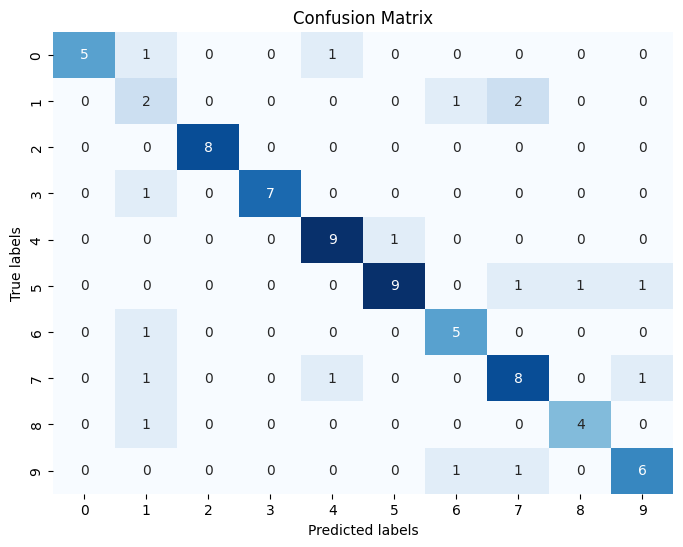
\includegraphics[width=1.0\textwidth]{figures/cv_metal_matrix.png}
    \caption{CV Metal Confusion Matrix}
    \label{cv_metal_matrix}
\end{figure}
From the confusion matrix for metals \ref{cv_metal_matrix}, metal 1 was difficult to recognize with many metals being misclassified as metal 1. 
\begin{figure}[h!]
  \centering
    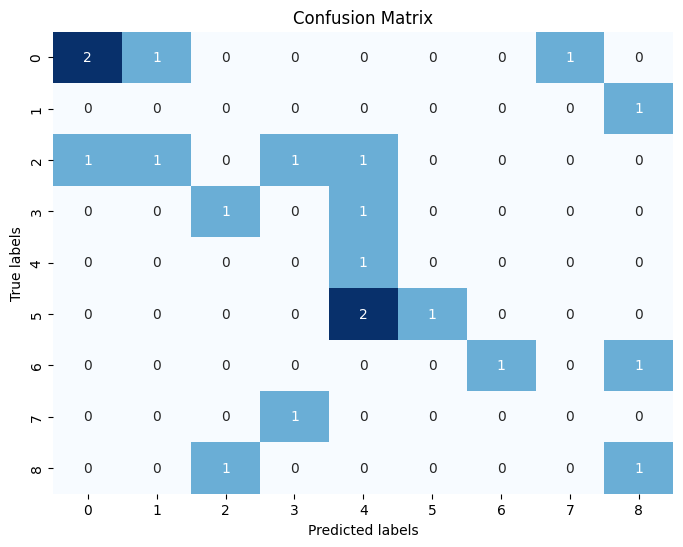
\includegraphics[width=1.0\textwidth]{figures/dpv_ligand_matrix.png}
    \caption{DPV Ligand Confusion Matrix}
    \label{dpv_ligand_matrix}
\end{figure}
\begin{figure}[h!]
  \centering
    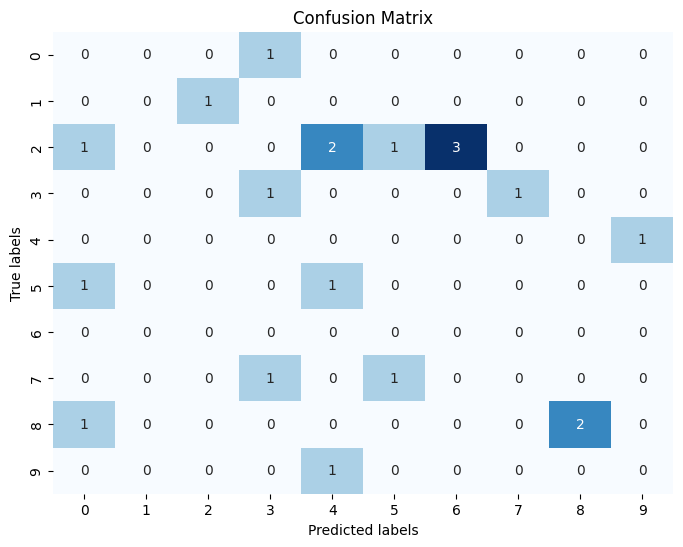
\includegraphics[width=1.0\textwidth]{figures/dpv_metal_matrix.png}
    \caption{DPV Metal Confusion Matrix}
    \label{dpv_metal_matrix}
\end{figure}
From the DPV confusion matrices seen in Figure \ref{dpv_metal_matrix} and Figure \ref{dpv_ligand_matrix}, it is hard to draw any definitive conclusions due to the dataset size. 
A major challenge in supervised learning is providing good examples during training. However, despite using a small dataset, these results are promising. 
